%!TEX root = GRoutes.tex
%%%%%%%%%%%%%%%%%%%%%%%%%%%%%%%%%%%%%%%%%%%%%%%%%%%%%%%%%%%%%%%%%%%%%%%
\chapter{GRoutes - alkalmazás bemutatása}\label{ch:ALAP}
%%%%%%%%%%%%%%%%%%%%%%%%%%%%%%%%%%%%%%%%%%%%%%%%%%%%%%%%%%%%%%%%%%%%%%%

\begin{osszefoglal}
	Ebben a fejezetben a GRoutes android applikációt fogom bemutatni úgy technikai, mint funkcionális szempontból.
	
\end{osszefoglal}

%%%%%%%%%%%%%%%%%%%%%%%%%%%%%%%%%%%%%%%%%%%%%%%%%%%%%%%%%%%%%%%%%%%%%%%
\section{Funkcionalitások}\label{sec:ALAP:adatelem}

\subsection{Bejelentkezés}

\begin{wrapfigure}{l}{0.4\linewidth}
	\centering
	\setlength{\abovecaptionskip}{0pt}
	\setlength{\belowcaptionskip}{0pt}
	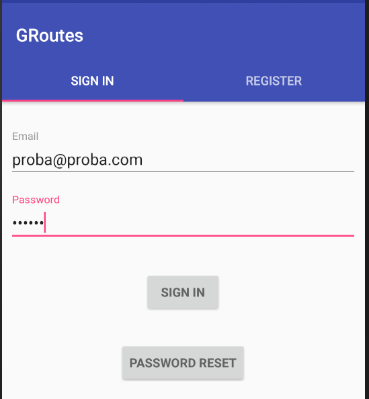
\includegraphics[width=0.4\textwidth]{images/login}
	\caption{Bejelentkezési felület\label{fig:ALAP:sm2}}
\end{wrapfigure}

Az alkalmazás elindítása után egy bejelentkezési felület fogadja a felhasználót. Itt kell megadni az e-mail címet, valamint a jelszót amivel a felhasználó regisztrált. Amennyiben elfelejtette a jelszavát, az "elfelejtett jelszó" gomb megnyomásával lehetőség van egy jelszó-visszaállító e-mail kiküldésére. 

Ha egy új felhasználó szeretné igénybe venni az applikáció szolgáltatásait, akkor regisztrálnia kell. Ezt megteheti a regisztráció lapra való navigálás után, melyet a cím megérintésével, vagy a képernyőn az ujjának balra történő húzásával érheti el. Az e-mail cím és az új jelszó megadása után, a felhasználó egyből a főmenübe érkezik, mindeközben azonban egy aktivációs e-mailt is kap arra a címére, amivel regisztrált. A későbbiekben csak akkor fog tudni bejelentkezni, ha a kapott emailben az URL%
\footnote{ %
	Uniform Resource Locator, más néven webcím
}  %
-re klikkelve aktiválja a felhasználóját.

\subsection{Főmenü}

A főmenüből négy különböző oldalra navigálhatunk tovább: a keresési felület, a régebbi keresések megtekintése, a kedvencek menedzselése, valamint a beállítások. Az ötödik (csoportok) oldal egy jövőbeli funkcionalitás kifejlesztésére van fenntartva.

\noindent
\begin{minipage}{\linewidth}
	\centering
	\begin{multicols}{2}
		
		\setlength{\abovecaptionskip}{10pt}
		\begin{Figure}
			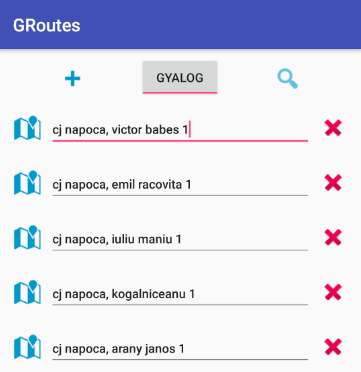
\includegraphics[width=\linewidth]{images/search}
			\captionof{figure}{Keresési felület
				\label{fig:search}}
		\end{Figure}
	
	\setlength{\abovecaptionskip}{10pt}
		\begin{Figure}
			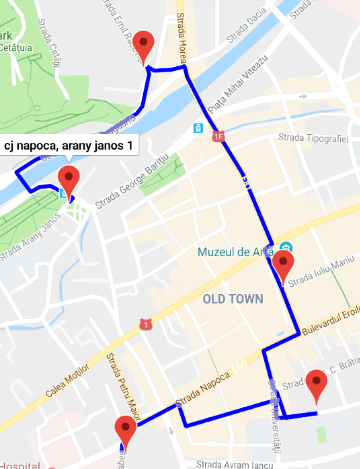
\includegraphics[width=\linewidth]{images/route}
			\captionof{figure}{Keresés eredménye 
			\label{fig:route}}
		\end{Figure}
	\end{multicols}
\end{minipage}

\subsection{Keresési felület}

Ezen a felületen van lehetőségünk útvonalak, helyszínek keresésére. A "+" gomb megjelenít egy új mezőt, ahol további címeket adhatunk meg. A "nagyító" gomb a térkép felületre navigál, és kirajzolja a tervezett útvonalat. A keresés elindítása előtt, minden cím mellett van egy "térkép" gomb, ennek segítségével tudjuk megnézni, hogy valóban az az a hely, amire gondoltunk.

\subsection{Kedvencek}
 
 Itt jelennek meg az általunk manuálisan elmentett utak, helyszínek. Minden bejegyzésnél négy gomb jelenik meg, ezeknek az funkcióik a következők:
 
 \begin{description}
 	\setlength{\itemsep}{0.04mm}
 	\item[térkép] -- megjeleníti a térkép felületet, ahol ráközelít a helyszín koordinátáira, vagy kirajzolja az útvonalat.
 	\item[nagyító] -- a keresési felülethez navigál és kitölti a keresési mezőket, az útvonal csomópontjaíval, így a felhasználó könnyedén módosíthatja útvonaltervét.
 	\item[ceruza] -- módosítja a bejegyzés nevét.
 	\item[szemetes veder] -- törli a bejegyzést, ezáltal az adatbázisból is törlődni fog.
 \end{description}

\subsection{Múltbeli keresések}

\begin{wrapfigure}{l}{0.4\linewidth}
	\centering
	\setlength{\abovecaptionskip}{0pt}
	\setlength{\belowcaptionskip}{-30pt}
	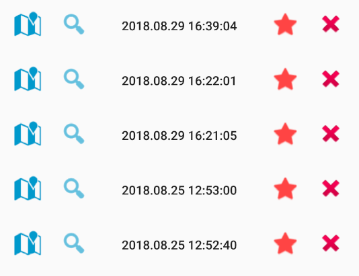
\includegraphics[width=0.4\textwidth]{images/history}
	\caption{Múltbeli keresések\label{fig:history}}
\end{wrapfigure}

A keresési felület eredményéül kapott útvonalak megjelennek a múltbeli keresések menüpont alatt, nevüket a keresési dátum és időpont alkotja. A bejegyzéseknél a "Kedvenceknél" tárgyalt gombok találhatóak, azonos funkcióval, azzal a kivétellel, hogy a "ceruza" gombot a "csillag" helyettesíti, melynek segítségével elmenthetünk egy útvonalat a kedvencek közé.

\subsection{Beállítások}

Itt ki tudjuk választani a limitet, hogy mennyi csomópont esetén, melyik algoritmust használja az alkalmazás. A megadott számnál kisebb vagy egyenlő számú csomópontok esetén a \(Concorde\) nevű egzakt megoldásokat nyújtó algoritmus fogja kiszámolni az ideális útvonalat. Ez az algoritmus a legpontosabb megoldásokat nyújtja, azonban az "utazó ügynök" problémájának komplexitása miatt, a csomópontok növekedésével, a végrehajtási idő is exponenciálisan növekszik. Amennyiben a felhasználó nagyon sok csomóponttal szeretne dolgozni, és fontosabb neki az, hogy belátható időn belül egy elfogadható megoldást kapjon, de nem probléma, ha nem a leghatékonyabb útvonal rajzolódik ki, akkor a megadott szám feletti mennyiségű csomópontok esetén, az applikáció egy úgynevezett \(greedy\)%
\footnote{ %
	mohó
}  %
 algoritmust fog használni. Ez nagyságrendekkel gyorsabb az exponenciálishoz viszonyítva, azonban nem minden esetben nyújtja a legjobb megoldást.

Ugyanitt megadhatjuk az alapértelmezett utazási módot, ami lehet gyaloglás, valamint vezetés.

Bár az egyszerűség kedvéért igyekeztem sok írás helyett szimbólumokat tenni a gombokra, de az applikációban található kevés szövegnek a nyelvét szintén itt lehet beállítani.

A térképpel, navigációval kapcsolatos paraméterek módosítására is van lehetőség, mint példaul az alapértelmezett nagyítás, a pozíció lekérésének gyakorisága, a térképre való automatikus ránagyítás és ennek centralizálásának a gyakorisága navigáció közben, valamint a megtett út kirajzolásának a mennyisége.

\subsection{Térkép felület}

Ez a felület akkor jelenik meg, amikor megérintjük a térkép gombot egy helyszín vagy egy útvonal mellett, valamint a keresési felület eredménye is itt rajzolódik ki.
Amennyiben egy helyszíntől érkezünk, megjelenik egy \(marker\)%
\footnote{ %
	jelző
}  %
az adott koordinátán.

A "csillag" gomb segítségével hozzáadhatunk egy helyszínt vagy egy útvonalat a kedvencekhez, ahol később visszanézhetjük, módosíthatjuk a nevét. Alapértelmezetten, a bejegyzések neve a keresési dátum és időpont lesz. A "nagyító" gomb segítségével visszatérhetünk a keresési felületre, így könnyedén módosíthatjuk tervezett útvonalunkat. Az "navigáció" gomb segítségével elkezdhetünk navigálni a tervezett útvonalon.

%%%%%%%%%%%%%%%%%%%%%%%%%%%%%%%%%%%%%%%%%%%%%%%%%%%%%%%%%%%%%%%%%%%%%%%
\section{Adatbázis}\label{sec:ALAP:adatelem}

 \begin{wrapfigure}{l}{0.5\linewidth}
	\centering
	\setlength{\abovecaptionskip}{0pt}
	\setlength{\belowcaptionskip}{0pt}
	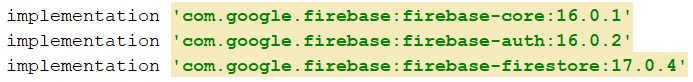
\includegraphics[width=0.5\textwidth]{images/firebase_gradle}
	\caption{A Firebase függőségei\label{fig:ALAP:sm2}}
\end{wrapfigure}

Adatbázisnak és az autentikáció menedzselésére Firebase-t használtam. Mielőtt bármilyen funkcióját is használhatnám ennek az applikációfejlesztési platformnak, be kellett jelentkezzek a Google felhasználómmal, készítenem kellett egy projektet, majd ezt a projektet össze kellett kapcsolnom magával az applikációval, amit fejleszteni szerettem volna. Van egy külön \(plugin\)%
\footnote{ %
	kiegészítés
}  %
 az \(Android Studio\)%
 \footnote{ %
 	fejlesztési környezet android applikációk számára
 }  %
-ban, melynek segítségével könnyedén létre lehet hozni a ezt kapcsolatot. Előtte azonban az applikáció Gradle állományába be kellett jelentsem a \(core\), \(auth\) és \(firestore\) modulokat, mint függőségeket.
 

 

\subsection{Autentikáció}

A web-es felületen engedélyeznem kellett az e-mail/jelszó bejelentkezést. Ugyanitt állítottam be, hogy biztonsági okokból maximum hány regisztrációt engedjen a rendszer óránként ugyanarról az IP címről, jelenleg ez 100. Regisztációkor generálódik egy egyedi felhasználói ID, ennek segítségével oldom meg, hogy minden felhasználó csak a saját adataihoz férjen hozzá. A bejelentkezés, regisztráció, jelszó visszaállító e-mail küldése műveleteket a FirebaseAuth \(singleton\)%
\footnote{ %
	egy tervezési minta, az adott osztályból egy és csak is egy objektumot lehet létrehozni
}  %
 osztály metódusaival oldottam meg.
 
 \begin{description}
 	\setlength{\itemsep}{0.04mm}
 	\item[createUserWithEmailAndPassword(email, jelszó)] -- létrehoz egy felhasználót az e-mail és jelszó karakterlánc paraméterek segítségével, majd sikeres válasz után be is jelentkezik
 	\item[signInWithEmailAndPassword(email, jelszó)] -- megpróbál bejelentkezni a megadott e-mail/jelszó kombinációval
 	\item[sendPasswordResetEmail(email)] -- küld egy jelszó visszaállító e-mailt a paraméterként megadott címre.
 \end{description}

Az aktivációs e-mail küldéséhez a FirebaseUser osztály insztanciájának a sendEmailVerification() metódusát használtam.

\subsection{Kollekciók, Dokumentumok}

\begin{wrapfigure}{l}{0.6\linewidth}
	\centering
	\setlength{\abovecaptionskip}{0pt}
	\setlength{\belowcaptionskip}{0pt}
	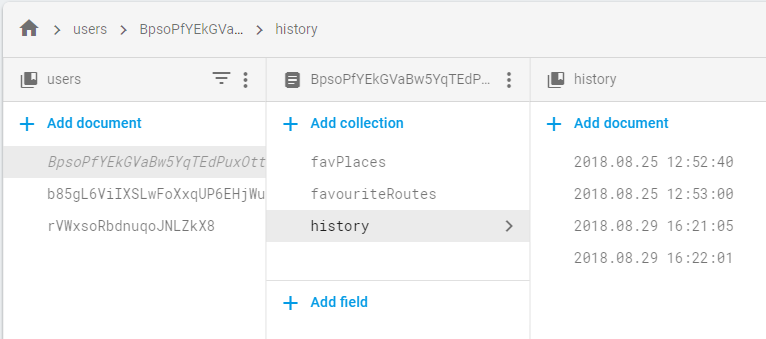
\includegraphics[width=0.6\textwidth]{images/firestore_colls}
	\caption{Firestore kollekciók\label{fig:ALAP:sm2}}
\end{wrapfigure}

A Firestore egy még Beta%
\footnote{ %
	még tesztelés alatt van
}  %
 verzióban levő no-sql, kulcs-érték párokra alapuló adatbázis, mely a Firebase platformon érhető el. Építőelemei a kollekciók és a dokumentumok, ezek váltakozva követik egymást, mivel egy kollekció csak dokumentumokat tartalmazhat, egy dokumentom viszont a kollekciók mellett adatokat (kulcs-érték párok) is tartalmazhat. 
 
 \begin{wrapfigure}{l}{0.6\textwidth}
 	\centering
 	\setlength{\abovecaptionskip}{0pt}
 	\setlength{\belowcaptionskip}{0pt}
 	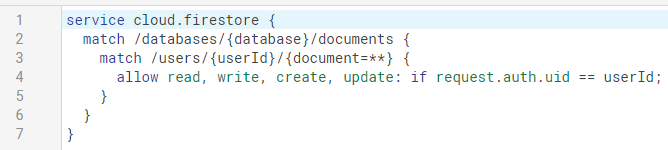
\includegraphics[width=0.6\textwidth]{images/firestore_rule}
 	\caption{Firestore szabály\label{fig:ALAP:sm2}}
 \end{wrapfigure}
 
Minden felhasználónak csak a saját dokumentumához van hozzáférése. Ezt egy úgynevezett szabály meghatározásával lehet elérni. Az adatbázis minden beérkező függvényhívást kiértékel a szabály alapján, és eldönti, hogy az adott kérésnek van-e elegendő jogosultsága. Amennyiben nincs, csak egy hibaüzenetet térít vissza.

 A GRoutes alkalmazás esetében a következőképpen építettem fel a struktúrát: van egy \(users\) kollekció, amely a felhasználókat tartalmazza. Minden felhasználói dokumentumnak az ID-ja megegyezik az UID%
\footnote{ %
	egyedi felhasználói ID, ami regisztrációkor generálódik
}  %
-val. A felhasználói dokumentumok a \(favPlaces\), \(favouriteRoutes\) és \(history\) kollekciókat tartalmazzák, melyek rendre megfelelnek a "kedvenc helyek", "kedvenc útvonalak" és "múltbeli útvonalak" fogalmaknak. Ezek a kollekciók tartalmazzák a különböző bejegyzéseknek (helyek, útvonalak) megfelelő dokumentumokat, melyek magukat az adatokat tartalmazzák. Az adatok sajátos entitás objektumok, melyeket a kódban, bizonyos szabályok alapján, de az én elképzelésem szerint hoztam létre. 


Egy út tartalmaz egy hely objektumokból álló tömböt a csomópontok számontartására, egy indexekből álló tömböt a csomópontok sorrendjének tárolására, valamint egy név mezőt.

Egy hely objektum tartalmaz egy-egy karakterlánc típusú név és cím mezőt, valamint egy GeoPoint objektumot, ami a hely főldrajzi szélességi és hosszúsági fokait tárolja.
 

%%%%%%%%%%%%%%%%%%%%%%%%%%%%%%%%%%%%%%%%%%%%%%%%%%%%%%%%%%%%%%%%%%%%%%%
\section{Osztályok}\label{sec:ALAP:adatelem}

\begin{figure}
	\centering
	\setlength{\abovecaptionskip}{-10pt}
	\setlength{\belowcaptionskip}{0pt}
	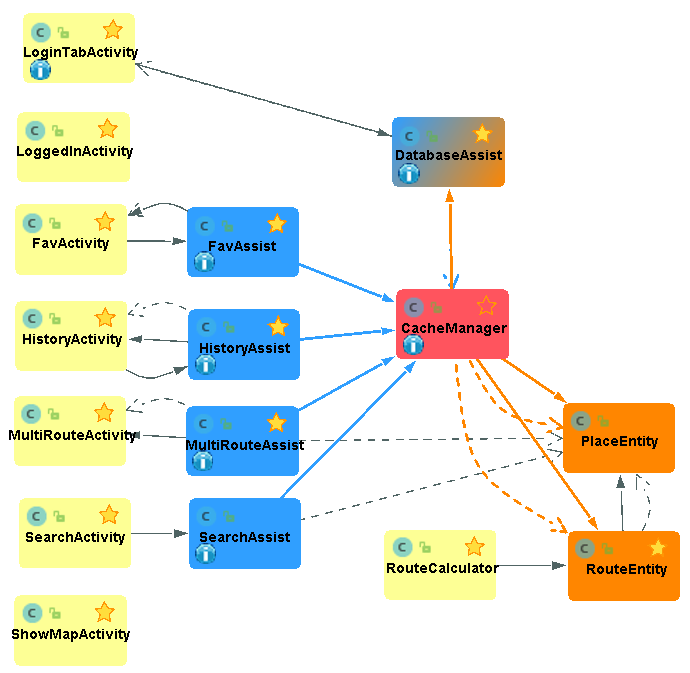
\includegraphics[width=1\textwidth]{images/class_diagram}
	\caption{Osztálydiagramm\label{fig:ALAP:sm2}}
\end{figure}

\subsection{Activity-k}\label{sec:ALAP:adatelem}

Egy android applikációban a UI%
\footnote{ %
	user interface - felhasználói felület
}  %
-t XML%
\footnote{ %
	Extensible Markup Language - Kiterjeszthető Jelölő Nyelv
}  %
állományok segítségével szerkeszthetjük meg, ezek azonban csak a külalakot adják meg. A háttérben végrehajtódó logikáért az Activity osztályok felelnek. A GRoutes alkalmazás különböző használati eseteihez más-más \(activity\) és XML állománypár tartozik.

\begin{description}
	\setlength{\itemsep}{0.04mm}
	\item[LoginTabActivity] -- ez a bejelentkezési felület, tehát ez fogad minket az alkalmazás indításakor. Itt történik az e-mail és a jelszó mezők validálása, a formátum ellenőrzése a bejelentkezési próbálkozás előtt. Használja a DatabaseAssist autentikációval foglalkozó metódusait, majd a válasz visszaérkezése után a LoggedInActivity-hez navigál.
	\item[LoggedInActivity] -- ez a főmenü. Amint beléptünk ide, a háttérben betöltjük a felhasználó adatait (múltbeli keresések, kedvencek). Innen tudunk tovább navigálni a főbb menüpontokhoz.
	\item[FavActivity] --  ez a "Kedvencek" felület. Mivel itt már komplexebb műveleteket kell végrehajtani, ezért azokat egy segédosztályba csoportosítottam, egy köztes réteget létrehozva a UI és az adatbázissal foglalkozó osztály között.
	\item[HistoryActivity] -- ez a "múltbeli keresések" menüpont, rendelkezik segédosztállyal 
	\item[MultiRouteActivity] -- ez felel az útvonalak kirajzolásáért, rendelkezik segédosztállyal 
	\item[SearchActivity] -- ez a keresés menüpont, rendelkezik segédosztállyal 
	\item[ShowMapActivity] -- a helyek megjelenítéséért felel
\end{description}

\subsection{Assist osztályok}\label{sec:ALAP:adatelem}

Általánosan, az alábbi segédosztályok végzik el a különböző Activity-k feladatait. Továbbá ők vannak kapcsolatban a CacheManager osztállyal, amely az adatok frissen tartásáért felel.

\begin{description}
	\setlength{\itemsep}{0.04mm}
	\item[FavAssist] -- feltölti adatokkal a "Kedvencek" felületet, dinamikusan beágyazza az XML-be a bejegyzéseket, továbbítja az activity módosítási, törlési szándékait a CacheManagernek
	\item[HistoryAssist] -- a FavAssist osztályhoz hasonló feladatokat végez el a HistoryActivity-nek. Egy múltbeli keresés kedvencekhez való hozzáadását is lemenedzseli
	\item[MultiRoutAssist] -- lekéri a csomópontok közti útvonalat a DirectionApi segítségével, majd kirajzolja a tervezett útvonalat a Polyline%
	\footnote{ %
		vonallánc
	}  %
 osztály használatával, továbbá a navigálásért is felel.
	\item[SearchAssist] -- feldolgozza a keresési címeket, majd a megfelelő adatstruktúrát lekommunikálja a CacheManager-nek
\end{description}

\subsection{Általános segédosztályok}\label{sec:ALAP:adatelem}

A fontosabb általános műveletek végrehajtására létrehoztam néhány Singleton mintára készült segédosztályt.

\begin{description}
	\setlength{\itemsep}{0.04mm}
	\item[DatabaseAssist] -- ez felel mindennemű Firebase-el kapcsolatos kommunikációért. Feladatai közé tartozik a regisztráció, bejelentkezés, az ezekkel kapcsolatos e-mail küldések, valamint a CRUD operációk elvégzése.
	\item[CacheManager] -- a központi adatmenedzselő osztály. Ő tölti be, aktualizálja, szolgálja ki a segédosztályokat az adatokkal, továbbítja kéréseiket a DatabaseAssist-nak. A LoginTabActivity kivételével csak ő áll kapcsolatban a DatabaseAssist segédosztállyal.
	\item[RouteCalculator] -- az optimális útvonal meghatározásáért felel (az utazó ügynök problémájának megoldása)\cite{pyconc}
\end{description}

\subsection{Entitás osztályok}\label{sec:ALAP:adatelem}

Az alkalmazás két nagyon fontos logikai struktúrát használ: helyek és útvonalak. Ezekkel több műveletet is kell végezni, mint például átalakítások, keresések, bizonyos paraméter alapján történő módosítások. Ezért számukra létrehoztam egy-egy entitás osztályt. 

A Firestore-ba való egyszerű mentés érdekében bizonyos kritériumoknak meg kell felelniük: rendelkezniük kell egy paraméter nélküli publikus konstruktorral, valamint az elmenteni kívánt attríbútumoknak publikus \(getter\) metódusokkal. Ezért azoknak az attribútumoknak a \(getter\) metódusait, amelyeket nem kívántam elmenteni, átneveztem úgy, hogy a \(ret%
\footnote{ %
	return - visszatérít
}  %
-\) prefixet használtam.

\begin{description}
	\setlength{\itemsep}{0.04mm}
	\item[PlaceEntity] -- három attribútuma van: egy String típusú név, egy GeoPoint típusú (magába foglalja a földrajzi szélességi és hosszúsági fokokat) helyszín és egy String típusú cím
	\item[RouteEntity] -- négy attribútuma van: egy String típusú ID (az adatbázisban történő azonosításra), egy String típusú név, egy egész számokból álló ArrayList típusú sorrend (a csomópontok bejárási sorrendjének tárolására) valamint egy helszínekből álló ArrayList típusú csomópont (csomópontok tárolása)
\end{description}



%%%%%%%%%%%%%%%%%%%%%%%%%%%%%%%%%%%%%%%%%%%%%%%%%%%%%%%%%%%%%%%%%%%%%%%
\section{Felmerülő problémák}\label{sec:ALAP:adatelem}


\subsection{Aszinkron függvényhívások}\label{sec:ALAP:adatelem}

Több olyan használati eset van, amikor egy bizonyos metódus az interneten keresztül kommunikál egy szerverrel. Ez mindig okozhat problémákat, de a szinkronhívásokat kivételkezeléssel egyszerűen meg lehet oldani. Több esetben, mint például a bejelentkezéskor vagy az adatok lekérdezésekor, a program nem vár a válaszra, hanem tovább végzi a következő műveleteket. Ez olyan helyzetekhez vezethet, hogy megnyitunk egy felületet és még nincsenek betöltve az adataink. 

Ezt a problémát úgy oldottam meg, hogy a DatabaseAssist osztály fog utólag jelezni annak az osztálynak ahonnan a kérés érkezett, amint választ kapott.


\subsection{Adatok aktualizálása az activity-k között}\label{sec:ALAP:adatelem}

Mivel az applikáció több különböző pontján van lehetőség az adatok hozzáadására, módosítására, törlésére, ezért fontos, hogy mindig, mindenhol a legfrissebb adatok birtokában legyünk.

Ezért vezettem be a CacheManager osztályt. Ez nem csak tárolja az aktuális adatokat, hanem az első lekérdezés kivételével, minden adatbázisműveletet lokálisan is elvégez, így a felhasználónak nem kell várnia, hogy a "múltbeli keresések" menüpont alatt megjelenjen a friss keresés, mivel azonnal hozzá lesz adva. Ellenkező esetben meg kéne várni, míg elmentjük az adatokat, majd lekérdezzük őket.

\subsection{Koordináta osztályok}

Egy földrajzi koordináta nem egy bonyolult adatszerkezet: tartalmaz egy földrajzi szélességi fokot, valamint egy hosszúsági fokot. Mégis három különböző osztályra volt szükség a reprezentálásához. 

\begin{description}
	\setlength{\itemsep}{0.04mm}
	\item[GeoPoint] -- a Firestore egyik beépített adattípusa, így az adatbázis, az egyszerű tárolás, valamint CRUD műveletekkel való kompatibilitás miatt szükség volt ennek használatára.
	\item[com.google.android.gms.maps.model.LatLng] -- a GoogleMap osztály használja. Ha egy \textit{Marker}-t szeretnénk egy térkép \textit{activity}-ben használni, akkor egy ilyen objektumot kell paraméterként átadjunk.
	\item[com.google.maps.model.LatLng] -- a Direction API, valamint a Distance Matrix API metódusaiban, paraméterként használt típus.
\end{description}

A \textit{Java} nyelvben nincs lehetőség egy importált osztály elnevezésére úgy, mint például \textit{Python}-ban. Ez azt eredményezte, hogy minden \textit{LatLng} típusú objektum létrehozásakor explicit meg kellett adni az egész csomag (\textit{package}) importálási ösvényét, mivel a két osztály neve megegyezik, és ez ambiguitást eredményez a \textit{compiler} számára.

